Il lavoro di tesi è stato strutturato in modo da poter condurre l'analisi della diffusione e la severità di istanze che possono causare technical debt sia nello stato dell'arte che nello stato della pratica.
Per questo motivo, il seguente lavoro inizia un'analisi preliminare della lettetura attraverso la conduzione di una \textit{Systematic Literature Review}.
Successivamente, al fine di ritrovare riscontro nello stato della pratica, è stata condotta un'investigazione al fine di estrarre il punto di vista degli sviluppatori sulla percezione, diffusione e severità di istanze di AI-Technical Debt, focalizzandosi dalla definizione dello stato dell'arte sulle istanze di AI Technical Debt che interagiscono con il codice e con l'architettura.

\section{Obiettivo di Ricerca}
Per ottenere più informazioni possibili sull'identificazione di AI-Technical Debt, è necessario estendere il lavoro di ricerca il più possibile. 

Lo scopo di questa tesi è quindi quello di definire una tassonomia utile ai professionisti che operano sui sistemi di Intelligenza Artificiale. Il risultato di questa tesi può essere quindi una guida utilizzabile per la identificazione di minacce che possono danneggiare la qualità del sistema basato su intelligenza artificiale.

Per raggiungere quest'obiettivo, sono state definite le seguenti research questions:
\break
\begin{rqbox}
\textbf{RQ1:} Come è definita in letteratura la tassonomia attuale degli AI Technical debt?
\end{rqbox}

\begin{rqbox}
\textbf{RQ2:} Qual è la percezione degli sviluppatori rispetto alla pericolosità dei technical debt in sistemi AI?
\end{rqbox}
\section{Systematic Literature Review}
Il processo di conduzione dell'analisi della letteratura è stato condotto seguendo le linee guida definite da Kitchenham \cite{kitchenhamSLR}:
\begin{enumerate}
    \item Definizione del processo di ricerca
    \item Identificazione della ricerca
    \item Validazione della qualità degli studi selezionati
    \item Estrazione e sintesi dei dati
    \item Reporting della revisione
\end{enumerate}

\subsection{Processo di Ricerca}

Il processo di ricerca per la conduzione dell'analisi della letteratura include la pianificazione di cinque passaggi utili alla collezione della letteratura.

\subsubsection{Definizione dell'obiettivo di ricerca}
Al fine di poter estrarre una tassonomia che possa essere di riferimento per i professionisti del software AI, l'obiettivo di ricerca dell'analisi della letteratura include lo scopo di identificare la presenza, l'impatto e la severità di istanze che possono causare AI-Technical Debt.
Inoltre, prevede di collezionare informazioni riguardanti possibili strategie di identificazione e di mitigazione della minaccia tramite tecniche di refactoring.


\subsubsection{Definizione delle Research Questions}
Dall'obiettivo definito, quindi sono state formulate le seguenti research question(RQs):
\hfill \break
\begin{rqbox}
\textbf{RQ1.1:} Quali tipologie di Technical Debt sono presenti nei sistemi AI?
\end{rqbox}
Molte tipologie di technical debt presenti in letteratura non hanno una definizione chiara
e precisa che ne permetta l’identificazione diretta nella pratica. È necessario, quindi,
seguire una strada analoga al lavoro introdotto da Ward Cunningham per la definizione
del Technical Debt \cite{Cunningham1992td}.
\hfill \break
\begin{rqbox}
\textbf{RQ1.2:} Quali sono gli approcci o i tool per identificare e mitigare TD nei sistemi AI?
\end{rqbox}
Al fine di fornire un metodo di riconoscimento ai professionisti del software AI delle istanze che possono causare technical debt, è necessario ricerca approcci che possano favorire l'identificazione. Questa parte del lavoro ha maggior successo se questi approcci sono stati implementati e distribuiti tramite la realizzazione di possibili tool, permettendo agli utenti della tassonomia di avere una tecnica automatizzata per l'identificazione.
Allo stesso modo, al fine di poter creare una linea guida utile ai professionisti del software AI, il lavoro di tesi si pone di ricercare possibili tecniche di refactoring utili a mitigare o ridurre il technical debt nei sistemi AI.

\subsubsection{Definizione del Coding Schema}

Al fine di pianificare lo schema di informazioni utile a indirizzare l'estrazione dei dati è necessario definire un processo di coding.
Il coding è il processo che comprende l'organizzazione di un grande ammontare di dati in piccoli frammenti, che favorisce l'estrazione delle informazioni.
Il processo prevede quindi l'assegnazione di codici, parole chiavi o frasi che identificano a quale problema o a quale argomento si riferiscono \cite{bailey2017guide}. 

La pianificazione del coding per il presente lavoro di tesi prevede innanzitutto la definizione di un coding schema preliminare, ossia un insieme di codici estratti dall'obiettivo di ricerca e dalle research questions formulate al fine di indirizzare la ricerca. Lo schema risultante deve poi essere verificato e raffinato attraverso l'applicazione dello schema su un sottoinsieme di articoli, così da ritrovare eventuali codici ancora non inclusi.
Il coding schema pianificato è definito in Tabella \ref{tab:coding_schema}.

\begin{table}[h!]
    \centering
    \begin{tabular}{|c|p{6cm}|}
        \multicolumn{2}{c}{\textbf{Coding schema}} \\
        
        \hline
        Scopo o topic & Informazioni relative allo scopo su cui opera l'articolo e il suo contributo di ricerca. \\
        \hline
        Tipologia di risorsa & Conferenza, Workshop o Journal e la tipologia dell'articolo.\\
        \hline
        Lista di istanze di technical Debt & Elenco dei nomi utilizzati per rappresentare le istanze di technical debt.\\
        \hline
        Definizioni di technical debt & Per ogni istanza riscontrata, definizione di essa. \\
        \hline
        Strategia di identificazione & Informazioni sulle strategie di identificazione delle istanze di technical debt. \\
         \hline
        Strategia di refactoring & Informazioni sulle strategie di refactoring delle istanze di technical debt. \\
         \hline
        Strumenti di identificazione & Informazioni sugli strumenti di identificazione delle istanze di technical debt. \\
        \hline
        Strumenti di refactoring & Informazioni sugli strumenti di refactoring delle istanze di technical debt. \\
        \hline
        Note & Informazioni aggiuntive non raggiungibili dal coding schema. \\
        \hline
    \end{tabular}
    \caption{Coding Schema pianificato per la Systematic Literature Review}
    \label{tab:coding_schema}
\end{table}


\subsubsection{Definizione del protocollo di revisione}
La revisione della letteratura prevede quindi una serie di attività che, a partire dalle sorgenti di dati, sarà possibile estrarre la serie di articoli che sono strettamente relativi all'obiettivo di ricerca definito.
Il protocollo di revisione quindi è utile alla conduzione sistematica della revisione per fornire una metodologia di selezione degli studi primari. La Figura \ref{fig:slr_process} definisce il protocollo di revisione adoperato per condurre lo studio, basato sulle linee guida definite da Kitchenham \cite{kitchenhamSLR}.
\begin{figure}
    \centering
    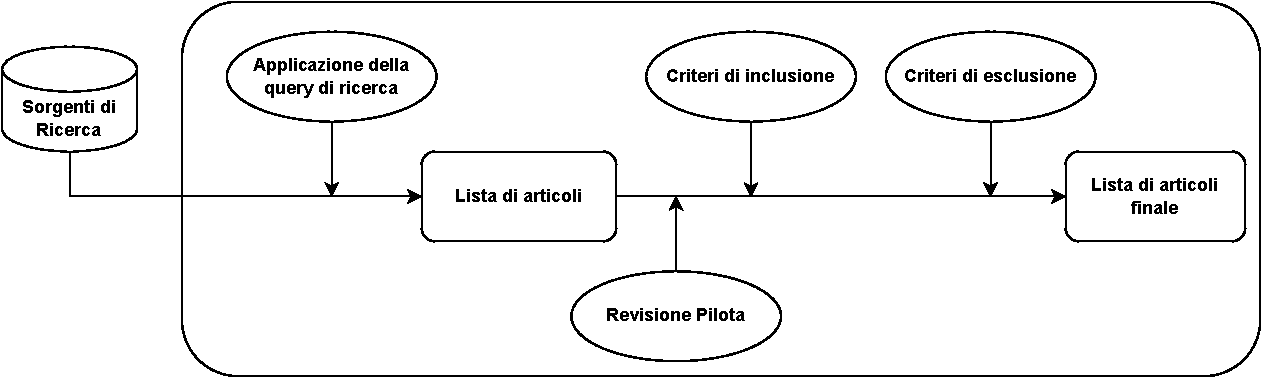
\includegraphics[width=1\textwidth]{Figure/Design/review_process.pdf}
    \caption{Protocollo di revisione della letteratura}
    \label{fig:slr_process}
\end{figure}
\subsection{Identificazione della Ricerca}
In questa sezione sono definiti le tecniche e le strategie utili alla selezione e la revisione degli articoli, seguendo il protocollo di revisione.
\subsubsection{Strategia di ricerca}
%sorgenti e search query
La strategia di ricerca include lo schema che definisce l'insieme delle sorgenti da analizzare, i termini di ricerca rilevanti, la definizione dei criteri di inclusione e di esclusione e infine la query di ricerca utilizzata.

Per questo lavoro sono state selezionate la lista di sorgenti bibliografiche rilevanti come suggerito da Kitchenham and Charters, definite anche come le più rappresentative del dominio di ingegneria del software \cite{Kitchenham2007}.
La lista include quindi: ACM Digital Library, IEEEXplore Digital Library, Web of Science e Scopus.

I termini di ricerca sono stati collezionati per poter rappresentare due sottogruppi di terminologie: una rappresentante le diverse tipologie di technical debt, l'altra rappresentante le diverse terminologie utilizzate per indicare l'intelligenza artificiale. La combinazione di questi due sottogruppi ha portato poi alla formulazione della seguente \textit{search query}:
\begin{quote}
   ("technical debt" $\vee$ "tech debt" $\vee$ "requirements debt" $\vee$ "data debt" $\vee$ "data smell*" $\vee$ "code debt" $\vee$ "build debt" $\vee$ "model debt" $\vee$ "documentation debt" $\vee$ "versioning debt" $\vee$ "defect debt" $\vee$ "configuration debt" $\vee$ "infrastructure debt" $\vee$ "design debt" $\vee$ "architecture debt" $\vee$ "architectural debt" $\vee$ "test debt" $\vee$ "defect debt" $\vee$ "abstraction debt" $\vee$ "ethics debt" $\vee$ "analysis debt" $\vee$ "" $\vee$ antipattern* $\vee$ anti-pattern* $\vee$ smell*) $\wedge$ ("machine learning" $\vee$ "deep learning" $\vee$ ai $\vee$ ml $\vee$ dl $\vee$ "artificial intelligence")
\end{quote}
E' stato utilizzato il carattere $"*"$ per indicare la possibile variazione dei termini (\eg variazione del termine da singolare a plurale).
Per incrementare la rilevanza degli articoli riscontrati, la search query è stata utilizzata sia sull'analisi del titolo sia sull'analisi dell'abstract dell'articolo.

\subsubsection{Definizione degli criteri di inclusione e esclusione}
Sono stati definiti i criteri di inclusione da essere applicati sia durante la fase di revisione iniziale in cui viene analizzato titolo e abstract dell'articolo (T\&A) sia durante la fase di revisione completa (F), come illustrato in Tabella \ref{tab:criteria}.

\begin{table}[h!]
    \centering
    \begin{tabular}{|c|p{6cm}|p{1.6cm}|}
    \hline
    \textbf{Criteria} & \textbf{Criterio di valutazione} & \textbf{Fase} \\ \hline 
    \multirow{2}{*}{\textbf{Inclusion}} & (I1) Articoli che definiscono le tipologie di technical Debt nei sistemi AI & Entrambi \\ \cline{2-3} 
    & (I2) Articoli che presentano approcci alla identificazione di technical Debt nei sistemi AI & Entrambi  \\\cline{2-3} 
    & (I3) Articoli che presentano approcci alla mitigazione di technical debt nei sistemi AI & Entrambi \\ \cline{2-3} 
    & (I4) Articoli che presentano tool per la identificazione di technical debt nei sistemi AI & Entrambi \\\cline{2-3}  
    & (I5) Articoli che presentano tool per la mitigazione di technical debt nei sistemi AI & Entrambi \\ \hline 
    \multirow{2}{*}{\textbf{Exclusion}} & (E1) Articoli non scritti interamente in lingua inglese & T\&A\\ \cline{2-3} 
    & (E2) Articoli che non stati soggetti a una peer review (i.e., blog, forum, book, book chapter, ...) &  T\&A\\ \cline{2-3} 
    & (E3) Articoli duplicati (da considerare solo la versione più recente) & T\&A \\ \cline{2-3} 
    & (E4) Position papers e work plans (i.e., articoli che non riportano risultati) & T\&A \\ \cline{2-3} 
    & (E5) Pubblicazioni non accessibili & T\&A \\ \hline
    \end{tabular}
    \caption{Criteri di inclusione e esclusione degli articoli in letteratura }
    \label{tab:criteria}
\end{table}

\subsection{Validazione della qualità degli studi selezionati}
Al fine di migliorare la qualità della metodologia di revisione adoperata, sono state utilizzate delle tecniche di validazione.
Per ridurre il fattore di soggettività all'interno del processo, è stato incluso un processo di \textit{Inter-rater assessment}.
In dettaglio, per la revisione è stata condotta da tre ricercatori, esperti di Technical Debt per i sistemi AI, al fine di valutare la search query e i criteri di inclusione e esclusione.
Il processo di revisione ha previsto un'analisi iniziale condotta da ogni ricercatore analizzando, tramite l'utilizzo dei criteri di inclusione ed esclusione, il titolo e l'abstract di ogni articolo.
A ogni articolo, quindi, viene assegnata la revisione da parte di due ricercatori, i quali dovranno esprimere il loro giudizio per l'inclusione (assegnato tramite il valore 1) o l'esclusione (assegnato tramite il valore 0).
In caso di disaccordo tra le valutazioni, è stato coinvolto il terzo ricercatore al fine di esprimere il voto finale.
Successivamente, è stato condotto un test pilota su un sottoinsieme di 6 articoli, revisionato da coppie di ricercatori.
Questo ultimo step ha permesso quindi di poter valutare la bontà del processo definito e di poter ottimizzare e raffinare i dettagli.



\section{Survey}
\subsection{Motivazione del survey}

Lo stato dell'arte attualmente non presenta un numero alto di risultati tale da poter estrarre una tassonomia completa dei possibili technical debt nei sistemi AI. 
E' necessario quindi estendere i confini delle informazioni estraibili allo stato della pratica.
L'utilizzo di un survey consente di poter estrarre il punto di vista e l'esperienza di esperti del settore di sistemi di intelligenza artificiale.
La loro esperienza sarà quindi utile per due principali motivazioni: ogni informazione estratta dal punto di vista degli esperti può fornire supporto a dettagliare la catalogazione e la tassonomia di AI Technical Debt; inoltre è possibile ricavare ulteriori informazioni riguardanti le necessità dell'esperto di sistemi AI al fine di poter migliorare la qualità dei propri sistemi. Le necessità evidenziate possono diventare quindi un punto di partenza per indirizzare la ricerca accademica verso soluzioni e strategie che rispondono alle esigenze dello stato della pratica.

\subsection{Obiettivo di Ricerca}
Al fine di poter contribuire a definire una tassonomia e una catalogazione ben dettagliata delle possibili istanze che possono causare AI Technical Debt, il lavoro di tesi si focalizza alla investigazione di due settori dettagliati di AI-Technical Debt: code debt e architectural debt.

L'obiettivo principale di ricerca per questo lavoro quindi è il seguente:
\begin{quote}
    \textit{Analizzare la diffusione, la severità e l'impatto di AI Technical Debt relativi al codice e all'architettura dei sistemi AI.}
\end{quote}

Per l'analisi di Ai Technical Debt relativi al codice e all'architettura sono stati estratti dalla letteratura le seguenti 9 istanze che possono causare Technical Debt, come raffigurato in Tabella \ref{tab:code_architectural smells}. 
\begin{table}[h]
    \centering
    \begin{tabular}{|c|c|}
    \hline
    \textbf{Debt type} & \textbf{Debt Instance}\\
    \hline
    \multirow{5}{*}{Architectural debt}
         & Jumbled Model Architecture \\
         & Pipeline Jungles \\
         & Multiple Language Smells \\
         & Undeclared Consumers \\
         & Correction Cascades \\
         \hline
    \multirow{4}{*}{Code debt}
         & Glue Code \\
         & Deep God File \\
         & Scattered Use of ML Libraries \\
         & Unwanted Debugging Code \\
        \hline
    \end{tabular}
    \caption{List of Code and Architectural Smell analyzed in this study}
    \label{tab:code_architectural smells}
\end{table}

\subsection{Research Questions}
Le domande di ricerca volte al raggiungimento dell'obiettivo sono definite seguendo la metodologia GQM \cite{Solingen}, utilizzato particolarmente nel campo di misurazione della qualità del software.
Questo è un metodo orientato agli obiettivi che utilizza un approccio top-down. 
La raffinazione dell'obiettivo viene quindi effettuata attraverso la formulazione delle domande per poi essere trasformate in metriche.
L'applicazione di questa metodologia nella ricerca corrisponde ad associare quindi le domande alle research questions formulate e le metriche associate al questionario \cite{Ciolkowski2003PracticalEI}.

Quindi, le research questions definite sono le seguenti:
\break
\begin{rqbox}
\textbf{RQ2.1:} Quali sono le tipologie di code debt e architectural debt più frequenti secondo la percezione degli sviluppatori AI?
\end{rqbox}

\begin{rqbox}
\textbf{RQ2.2:} Quali sono le tipologie di code debt e architectural debt più problematiche secondo la percezione degli sviluppatori AI?
\end{rqbox}


\begin{rqbox}
\textbf{RQ2.3:} Qual è l'impatto causato dai code debt e architectural debt secondo la percezione degli sviluppatori AI?
\end{rqbox}

\begin{rqbox}
\textbf{RQ2.4:} Quali sono le strategie utilizzate dagli sviluppatori AI per l'identificazione e la mitigazione di code debt e architectural debt?
\end{rqbox}





\subsection{Design del Survey}
La conduzione del presente studio ha previsto lo svolgimento di differenti fasi, al fine di massimizzare l'affidabilità delle risposte ricevute.


\subsection{Design e configurazione dell'esperimento}
Lo studio prevede di analizzare in dettaglio il punto di vista degli sviluppatori sulla presenza, la severità e l'impatto di 9 istanze che possono causare AI Technical Debt.
Al fine di poter aumentare il livello di comprensibilità da parte degli sviluppatori, il tipo di esperimento condotto è basato sulla metodologia di \textit{Experimental Vignette Study} introdotta da Atzmuller et al. \cite{AtzmullerVignetta}. Questa tipologia di esperimento prevede la rappresentazione degli oggetti sperimentali tramite vignetta.
Una vignetta è una breve e dettagliata descrizione di una persona, oggetto o situazione che rappresenti una combinazione di caratteristiche.
La scelta di quest'approccio deriva dalla sua capacità tramite descrizione di rappresentare scenari realistici, dando la possibilità ai partecipanti di comprendere i dettagli.
Le definizioni fornite dalla letteratura per la rappresentazione delle 9 istanze di AI Technical Debt sono state quindi utilizzate per la creazione delle vignette, come raffigurato in Tabella \ref{tab:aitd_c_vignetta} e in Tabella \ref{tab:aitd_a_vignetta}.

\begin{table}[h]
    \centering
    \scriptsize
    \begin{tabular}{|l|p{6cm}|}
    \hline
        \textbf{AiTechnicalDebt} & \textbf{Vignetta}\\
        \hline
         Glue Code & Suppose that you are working on a machine learning application code. During the development, you notice inside the code a popular general-purpose library that contains a lot of different models. You have seen that the whole library is imported inside the system and the application contains a big part of code that allows you to fit data from the library to the specific model that you have.\\
             \hline
         Deep God File & Suppose that you are working on a machine learning application. You try to identify and highlight the code of specific functionality of the application. You notice that the entire application is encapsulated in a single file that contains all the operations of the application. So, you attempt to highlight the part of the code that you need but it's very hard to perceive it.\\
             \hline
         Scattered Use of ML Libraries & Suppose that you are working on a machine learning application. You see in your application that a part of the team introduced many libraries for the steps of the pipeline, without a cohesive manner.\\
            \hline
         Unwanted Debugging Code & Suppose that you are working on the maintenance of a machine learning application. You see in your application that a part of the team introduced some debugging code, for example, an intermediate sequence of loggers.\\
         \hline
    \end{tabular}
    \caption{Rappresentazione delle istanze di AI Technical Debt di codice attraverso la metodologia della vignetta}
    \label{tab:aitd_c_vignetta}
\end{table}

\begin{table}[h!]
    \centering
    \scriptsize
    \begin{tabular}{|l|p{6cm}|}
    \hline
        \textbf{AI TechnicalDebt} & \textbf{Vignetta}\\
        \hline
         Jumbled Model Architecture & Suppose that you are working on a machine learning application. After seeing the machine learning pipeline, you try to identify and highlight the code that reflects the step of the machine learning pipeline. You notice that all the stages of the machine learning pipeline are all together and it’s difficult to recognize each stage.\\
             \hline
         Pipeline Jungles & Suppose that you are working on a machine learning pipeline application. During the pipeline definition of the model, you see that each part of the team adds several steps for each phase of the pipeline, and you notice that the entire pipeline starts growing more.\\
             \hline
         Multiple Language Smells & Suppose that you are working on the machine learning application code. During the development, you notice that part of your team introduced a library that allows you to resolve an important task of the Machine Learning Pipeline. On the other side, you see that this component is written in a different language from the rest of the application.\\
             \hline
         Undeclared Consumers & Suppose that you are working on the maintenance and updating of a machine learning model. In order to modify the model, you want to know what applications use the output data of your model. You discover through the access control that there are some unknown applications that collect the data from the model.\\
             \hline
         Correction Cascades & Suppose that you are working on a new machine learning application and your team wants to use a built model X to resolve a slightly different problem. So, your team created a model Y that takes X's output in input and makes a hotfix in order to fit the solution of the new problem.\\
             \hline
    \end{tabular}
    \caption{Rappresentazione degli AI-Technical Debt architetturali attraverso la metodologia della vignetta}
    \label{tab:aitd_a_vignetta}
\end{table}


Per la progettazione dell'esperimento, al fine di ottenere un numero sufficiente di risposte da ogni partecipante senza oltrepassare i limiti del numero di domande ammissibili, è stato deciso di adoperare una strategia di tipo \textit{mixed-design} \cite{AtzmullerVignetta}.
Le diverse istanze di Ai Technical Debt sono state suddivise in tre gruppi: A,B e C.
\begin{itemize}
    \item Gruppo A: Glue Code, Multiple Language Smell, Undeclared Consumers.    \item Gruppo B: Pipeline Jungles, Correction Cascades, Scattered Use of ML Libraries.
    \item Gruppo C: Jumbled Model Architecture, Unwanted Debugging Code, Deep God File.
\end{itemize}

%Rappresentazione degli oggetti sperimentali.
\subsubsection{Prescreening}
E' stato elaborato un questionario iniziale per raccogliere le informazioni sulle competenze dei partecipanti, al fine di garantire che il partecipante possa essere considerato un esperto del contesto e le sue risposte possano avere una validità.
In particolare, il questionario preliminare di \textit{prescreening} è suddiviso in due sezioni: una sezione che contiene domande sulle informazioni professionali e sulla sua esperienza negli ambiti relativi al contesto; la sezione successiva relativa all'esperienza del partecipante sui sistemi di intelligenza artificiale, cercando di estrarre su quale parte del sistema il partecipante ha maggiore focus.

La prima sezione quindi, richiede l'inserimento dal partecipante di informazioni relative alla dimensione dell'azienda e il suo ruolo nell'azienda, per poi approfondire le conoscenze nei campi della programmazione, ingegneria del software e intelligenza artificiale. Le domande relative alle conoscenze saranno poi analizzate attraverso l'utilizzo di una scala likert per poter rappresentare il livello di competenza, come raffigurato in Tabella \ref{tab:info_prof}.
\begin{table}[h!]
    \centering
    \begin{tabular}{|l|p{7cm}|c|}
        \hline
        \textbf{ID} & \textbf{Domanda} & \textbf{Tipologia di Domanda}\\
        \hline
        \hline
        PD1 & Qual'è il tuo ruolo nella compagnia?  & Caselle di controllo\\
        \hline
        PD2 & Quanti anni di esperienza hai nel tuo ruolo?  & Caselle di controllo\\
        \hline
        PD3 & Definisci il tuo livello di conoscenza di programmazione?  & Scala Likert\\
        \hline
        PD4 & Definisci il tuo livello di conoscenza di ingegneria del software?  & Scala Likert\\
        \hline
        PD5 & Definisci il tuo livello di conoscenza di intelligenza artificiale?  & Scala Likert\\
        \hline
    \end{tabular}
    \caption{Domande sulle informazioni professionali del partecipante}
    \label{tab:info_prof}
\end{table}
Nella seconda sezione, dopo aver fornito un'illustrazione raffigurante una tipica pipeline di un'applicazione AI, è stato chiesto al partecipante una serie di domande con lo scopo di comprendere quale fosse la parte del sistema dove egli ha maggiore interazione.
Inoltre, in questa sezione è stata aggiunta una domanda di controllo dell'attenzione al fine di controllare la consistenza delle risposte e verificare che il partecipante abbia risposto con interesse, come raffigurato in Tabella \ref{tab:info_ai}.
In particolare, l'ultima domanda controlla la conoscenza del partecipante dei sistemi AI, richiedendo di indicare in quale fase si applicano le tecniche di bilanciamento.


\newlength{\thickarrayrulewidth}
\setlength{\thickarrayrulewidth}{2\arrayrulewidth}
\begin{table}[h!]
    \centering
    \begin{tabular}{|c|p{7cm}|c|}
        \hline
        \textbf{ID} & \textbf{Domanda} & \textbf{Tipo Domanda}\\
        \hline
        \hline
        \multicolumn{3}{|c|}{\textbf{In quali di queste attività hai esperienza?}}\\
        \hline
        PD6 & Data ingestion, data aggregation o altre pratiche di data preparation  & Scala Likert\\
        \hline
            PD7 & Model selection e model training  & Scala Likert\\
        \hline
        PD8 & Model validation, review process e improving model  & Scala Likert\\
        \hline
        PD9 & Monitoring and maintenance and deployment plan  & Scala Likert\\
        \hline
        PD10 & Utilizzare librerie di Machine Learning e esecuzione del modello  & Scala Likert\\
        \hline
        \hline
        PD11 & Quale di queste attività raffigura meglio le tue attività di lavoro? & Scelta Multipla\\
        \hline
        PD12 & In quale parte del dataset applicheresti la tecniche di bilanciamento dei dati? & Caselle di Controllo*\\
        \hline
        \multicolumn{3}{c}{* = Domanda per il controllo dell'attenzione}
    \end{tabular}
    \caption{Domande sulle conoscenze dei sistemi di Intelligenza Artificiale del partecipante}
    \label{tab:info_ai}
\end{table}

La formulazione di queste domande ha lo scopo di poter andare a selezionare i partecipanti che realmente hanno esperienza sul campo dei sistemi AI.
Quindi, la selezione di questi partecipanti viene effettuata in base a una serie di criteri:
\begin{itemize}
    \item Il partecipante deve aver risposto correttamente alla domanda PD12.
    \item Il partecipante deve avere una conoscenza di programmazione (PD3) almeno pari a Basic (2/5).
    \item Il partecipante deve avere una conoscenza di ingegneria del software (PD4) o intelligenza artificiale (PD5) almeno pari a Intermediate (3/5).
    \item Se il partecipante rispetta il requisito precedente, il partecipante deve avere nell'altra disciplina una conoscenza almeno pari a Basic (2/5).
    \item Il partecipante deve avere conoscenza di monitoraggio, manutenzione e sviluppo del modello (PD9) almeno pari a Intermediate (3/5) oppure una conoscenza di utilizzo di librerie di machine learning (PD10) almeno pari a Intermediate (3/5).
\end{itemize}


\subsubsection{Domande del questionario}

Il risultato della fase di progettazione ha previsto di inserire sezioni su diversi aspetti per completare le informazioni sulla conoscenza e l'esperienza del partecipante.
In particolare, sono state definite due tipologie di sezioni: la prima intende completare l'estrazione delle informazioni riguardanti le attività professionali del partecipante già definite nel questionario di prescreening. Per questo motivo è stato deciso di richiedere al partecipante informazioni riguardanti la dimensione del team e la dimensione dell'organizzazione in cui esibisce la professione, come raffigurato in Tabella \ref{tab:info_prof_add}.

\begin{table}[h]
    \centering
    \begin{tabular}{|l|p{6.8cm}|c|}
        \hline
        \textbf{ID} & \textbf{Domanda} & \textbf{Tipologia di Domanda}\\
        \hline
        S1D1 & Da quanti membri è composto il tuo team?  & Caselle di controllo\\
        \hline
        S1D2 & Da quanti membri è composta la tua organizzazione?  & Caselle di controllo\\
        \hline
    \end{tabular}
    \caption{Domande aggiuntive sulle informazioni professionali del partecipante}
    \label{tab:info_prof_add}
\end{table}

Successivamente, sono state progettate la serie di domande in base agli obiettivi di ricerca definiti.
In particolare, per ogni istanza di AI-Technical Debt definito, è stato richiesto di fornire informazioni riguardanti ogni domanda di ricerca definita, ovvero attraverso la seguente categorizzazione:
\begin{itemize}
    \item Domande riguardanti la frequenza e la severità di AI-Technical Debt.
    \item Domande riguardanti l'impatto di AI-Technical Debt.
    \item Domande riguardanti le possibili strategie e tool di identificazione e refactoring utilizzati per rilevare AI-Technical Debt.
\end{itemize}

Per poter rispondere alla $RQ_1$ e alla $RQ_2$, le domande progettate relative alla frequenza di AI Technical Debt e la loro severità sono 5, come raffigurato in Tabella \ref{tab:q_freq_severity}.
Le domande chiedono esplicitamente al partecipante se la possibile situazione analizzata tramite vignetta, può risultare problematica all'interno di un sistema AI e se, nella loro esperienza, si sono ritrovati in una situazione simile.
Successivamente, al fine di avere informazioni aggiuntive sulla severità della situazione descritta, viene chiesto ai partecipanti l'ammontare di sforzo necessario al fine di poter identificare la situazione e effettuare operazioni di refactoring. 
\begin{table}[h]
    \centering
    \begin{tabular}{|l|p{6.8cm}|c|}
        \hline
        \textbf{ID} & \textbf{Domanda} & \textbf{Tipologia di Domanda}\\
        \hline
        S2D6 & Quanto spesso ritrovi questa situazione all'interno del progetto?  & Scala Likert\\
        \hline
        S2D1 & Quanto trovi problematica questa situazione?  & Scala Likert\\
        \hline
        S2D2 & Perchè può essere (o può non essere) problematica?  & Risposta testuale\\
        \hline
        S2D5 & Quanto sforzo pensi sia necessario al fine di identificare questa situazione?  & Scala Likert\\
        \hline
        S2D7 & Quanto sforzo pensi sia necessario al fine di effettuare refactoring, mitigazione o miglioramenti per questa situazione?  & Scala Likert\\
        \hline
    \end{tabular}
    \caption{Domande aggiuntive sulle informazioni professionali del partecipante}
    \label{tab:q_freq_severity}
\end{table}

Per rispondere alla $RQ_3$, le domande relative all'impatto sono basate su tre importanti aspetti di qualità:
\begin{itemize}
    \item Impatto sulle altre componenti(I)
    \item Comprensibilità (C)
    \item Evoluzione (E)
    \item Performance (P)
    \item Accoppiamento (A)
    \item Manutenibilità (M)
\end{itemize}

Dalla definizione di questi 3 aspetti di qualità, sono state formulate le seguenti domande:

\begin{table}[h]
    \centering
    \begin{tabular}{|l|p{6cm}|c|}
        \hline
        
        \textbf{ID} & \textbf{Domanda} & \textbf{Tipologia di Domanda}\\
        \hline
        \hline
        \multicolumn{3}{|c|}{Penso che questa situazione possa ...}\\
        \hline
        S2D9 & ... danneggiare le altre componenti dell'applicazione. (I)  & Scala Likert\\
        \hline
        S2D10 & ... rendere il livello di interpretabilità e comprensione più complesso per il modello. (C)  & Scala Likert \\
        \hline
        S2D11 & ... rendere difficile l'evoluzione dell'applicazione. (E)& Scala Likert\\
        \hline
        S2D12 & ... impattare e decrementare le perfomance del modello. (P)& Scala Likert\\
        \hline
        S2D13 & ... incrementare il numero di dipendenze e aumentare l'accoppiamento. (A) & Scala Likert\\
        \hline
        \hline
        S2D14 & ... incrementare i costi e lo sforzo di manutenzione dell'applicazione. (M) & Scala Likert\\
        \hline
    \end{tabular}
    \caption{Domande aggiuntive sulle informazioni professionali del partecipante}
    \label{tab:q_freq_impact}
\end{table}


Per poter rispondere alla $RQ_4$ infine, ovvero trovare le possibili strategie e tool utilizzati nello stato della pratica al fine di effettuare identificazione e refactoring, il questionario prevede l'inclusione di una domanda sulla modalità di approccio all'identificazione per indirizzare il partecipante a rispondere, e poi maggiori approfondimenti, come descritto nella Tabella \ref{tab:q_identification}.

\begin{table}[h]
    \centering
    \begin{tabular}{|l|p{6.8cm}|c|}
        \hline
        \textbf{ID} & \textbf{Domanda} & \textbf{Tipologia di Domanda}\\
        \hline
        S2D3 & Quali sono le tue pratiche utili a identificare la situazione descritta?  & Caselle di Controllo\\
        \hline
        S2D4 & Puoi specificare con maggiore dettaglio le tue pratiche di identificazione?  & Risposta testuale\\
        \hline
        S2D8 & Come effettui le pratiche di refactoring per la situazione descritta? & Risposta testuale\\
        \hline
    \end{tabular}
    \caption{Domande sulle strategie di identificazione e refactoring utilizzate dal partecipante}
    \label{tab:q_identification}
\end{table}
\subsection{Validazione del Survey}
Al fine di poter analizzare e evitare la presenza di potenziali minacce alla validità dell'esperimento, è stato deciso di realizzare una simulazione pilota di partecipanti esperti del settore. E' stata quindi inclusa la partecipazione di 6 ricercatori e esperti dell'Università degli studi di Salerno al fine di valutare la bontà del questionario.
I risultati hanno migliorato la qualità descrittiva delle domande e, in particolare, la qualità descrittiva delle vignette utilizzate per la rappresentazione delle istanze di AI-Technical Debt.

\subsection{Reclutamento dei partecipanti}
Lo studio è mirato all'acquisizione del punto di vista di figure professionali che hanno esperienza con i sistemi di intelligenza artificiale.
Per questa motivazione, il questionario è stato indirizzato verso i professionisti che hanno esperienza di ingegneria del software e di intelligenza artificiale nel campo aziendale.

Il possibile rischio affrontato durante la fase di reclutamento dei partecipanti è stata la possibilità di non ottenere un numero sufficienti di risposte utili a raggiungere i nostri obiettivi di ricerca. 
Il reclutamento dei partecipanti è stato quindi effettuato tramite la piattaforma \textit{Prolific}, la quale permette di indirizzare il questionario proposto verso i professionisti del settore desiderato, attraverso l'utilizzo di filtri sul profilo.
In particolare, nel nostro esperimento sono stati reclutati per rispondere alle domande di prescreening 500 partecipanti, i quali rispettassero i seguenti criteri iniziali:
\begin{itemize}
    \item Esperienza in programmazione.
    \item Conoscenza delle tecniche di sviluppo software (\eg Monitoraggio o testing).
\end{itemize}
Inoltre, il processo di prescreening descritto precedentemente aiuterà ad avere una ulteriore selezione sui partecipanti che hanno l'esperienza più consona al raggiungimento dell'obiettivo di ricerca.

Dall'insieme dei partecipanti risultanti idonei dopo il processo di prescreening, lo studio prevede di condurre l'investigazione tramite survey suddividendo il nuovo insieme di partecipanti nei tre gruppi definiti per le istanze di AI Technical Debt.

In dettaglio, a ogni partecipante è stato assegnato una combinazione di due gruppi di istanze al fine di aumentare il numero di risposte, come raffigurato in Tabella \ref{tab:design_experiment}.

\begin{table}[h]
    \centering
    \begin{tabular}{|c|c|}
        \hline
        \textbf{Partecipanti} & \textbf{Istanze di Ai Technical Debt}  \\
        \hline
        Gruppo 1 & Gruppo A+B \\
        Gruppo 2 & Gruppo B+C \\
        Gruppo 3 & Gruppo A+C \\
        \hline
    \end{tabular}
    \caption{Suddivisione dei partecipanti per gruppi di Ai-Technical Debt}
    \label{tab:design_experiment}
\end{table}

I partecipanti saranno ricontattati quindi tramite la piattaforma \textit{Prolific} al fine di rispondere e sottomettere il nuovo questionario.

